% main.tex
\documentclass[12pt]{article}

\usepackage[margin=1in]{geometry}
\usepackage{natbib}
\usepackage{hyperref}
\hypersetup{
  colorlinks=true,
  linkcolor=blue,
  filecolor=magenta,
  citecolor=blue,
  urlcolor=cyan,
  pdftitle={How to Study Boundary Phenomena},
  pdfpagemode=FullScreen,
}
\usepackage[T1]{fontenc}
\usepackage[utf8]{inputenc}
\usepackage{amsmath}
\usepackage{graphicx}
\usepackage{tipa}

\title{Language as a Stack of Homeostatic Property-Cluster Kinds: From Phonemes to Constructions}
\author{Brett Reynolds}
\date{}

\begin{document}
\maketitle

\begin{abstract}
\noindent Categories in language are stable enough to support reliable inference yet flexible enough to drift, diversify, and admit exceptions. I argue that many linguistic categories---phonemes, lexemes, and language-internal constructions---are \textsc{homeostatic property-cluster} (HPC) kinds: probabilistic clusters of articulatory, acoustic, semantic, and distributional properties stabilized by identifiable mechanisms at biological, cognitive-developmental, and sociocultural levels. Building on Miller's account of words as HPCs, which rejects essence-based individuation in favor of mechanism-indexed clusters, and on recent evidence that phonemes function as culturally maintained cognitive tools, I generalize the HPC template across linguistic levels and supply operational diagnostics and compact case studies. The diagnostics are (i) a projectibility test: tokens of a proposed kind support out-of-sample inferences about form/meaning/distribution; and (ii) a homeostasis test: specific stabilizers can be named and their property covariance shown. I demonstrate these with (A) phoneme typology (inventory ridgelines by family and the probability of /y/ increasing with vowel-inventory size), (B) a word-level diachrony showing distributional ``cluster cohesion'' under semantic drift, and (C) an English construction (\emph{let alone}), with cue bundling and cross-corpus replication. I also delimit non-HPCs: one-off items (nonce coinages), analyst-level macro-categories (e.g., cross-linguistic ``resultative'' as a single kind), and negative/complement classes. The result is a general method for deciding when a linguistic category earns kindhood by HPC lights, why some categories travel well across speakers and time, and where category proposals fail. The approach integrates philosophy-of-science clarity about kinds with quantitative, reproducible analyses familiar to cognitive science \citep{Miller2021WordsSpeciesKinds,Ekstrom2025PhonemeTool}.
\end{abstract}

\section*{Outline}
\begin{enumerate}
  \item \textbf{Introduction:} Frame the problem of category stability without essences; motivate HPC kinds for language; preview diagnostics and contributions; position relative to \citet{Miller2021WordsSpeciesKinds} and the ``phoneme as cognitive tool'' results \citep{Ekstrom2025PhonemeTool}.
  \item \textbf{Framework and diagnostics:} Define HPC for linguistic categories; state projectibility and homeostasis tests; map stabilizers (biophysical, developmental, sociocultural) and show how they correspond to the cognitive-tool criteria.
  \item \textbf{Case A (phoneme, positive):} Replicate family-wise inventory ridgelines and model $P(\text{/y/}\mid \text{vowel-inventory size})$; interpret patterns as signatures of homeostasis (quantal regions, dispersion), with developmental and normative scaffolding.
  \item \textbf{Case B (word, positive under drift):} One lexeme with documented semantic change (distributional neighborhood cohesion across decades; held-out prediction) consistent with Miller's mechanism-first individuation of word-kinds.
  \item \textbf{Case C (construction, positive):} \emph{let alone} as an HPC: cue bundling, collostructional profiles, and cross-corpus replication; stabilize via frequency, redundancy, and local performance standards.
  \item \textbf{Failures:} Too thin (nonce items, performance blends), too fat (global ``resultative''/``ditransitive''), and negative/complement classes (``ungrammatical strings''); reserve kindhood for local equilibria.
  \item \textbf{Predictions and disconfirmers:} Perturbation and scaling predictions; what would falsify an HPC claim at each level.
  \item \textbf{General discussion:} What HPC buys cognitive science; limits and next steps (developmental evidence; iterated-learning models; cross-linguistic extension).
\end{enumerate}

\section{Introduction}
Language presents a familiar problem for cognitive science: the categories we rely on to speak and understand are stable enough to underwrite reliable inference yet flexible enough to drift and diversify. An attractive middle ground---originating in Boyd’s account of \textsc{homeostatic property–cluster} (HPC) kinds---treats many scientific and social categories as probabilistic clusters stabilized by mechanisms that keep enough of the cluster together for inductive use \citep{Boyd1991Enthusiasm,Boyd1999Homeostasis}\footnote{For the first explicit HPC formulation (applied to moral terms), see \citet[§3.8]{Boyd1988MoralRealist}. For an explicit allowance that social mechanisms can underwrite homeostasis, see \citet{Boyd2000Workmanship}.}. On that understanding, I treat phonemes, words, and language-internal constructions as a posteriori kinds maintained by identifiable stabilizers.

For words, \citet{Miller2021WordsSpeciesKinds} develops this stance, rejecting essence-based individuation in favor of mechanism-indexed clusters that are historically delimited and population-relative. On this view, word-kinds earn their status because internal (cognitive) and external (normative) mechanisms sustain covarying properties---pronunciation, orthography, meaning, distribution---so that speakers can project from attested tokens to new ones.


At the phonological level, recent work argues that phonemes are culturally maintained \textsc{cognitive tools} anchored in articulatory and auditory constraints. Two quantitative signatures exemplify the sort of measurable ``homeostasis'' HPC requires: family-wise \textsc{ridgelines} of inventory sizes showing most languages cluster roughly between 20 and 50 segments, and a scaling curve in which the probability that a language includes /y/ rises with vowel-inventory size, while /i/ remains common even in small systems. Both patterns are presented with explicit methodological detail and tied to biophysical and efficiency pressures, and a compact checklist of tool criteria summarizes the stabilizers involved \citep[Fig.\,1 p.\,4; Fig.\,2 p.\,7; Table\,1 p.\,14]{Ekstrom2025PhonemeTool}. These are precisely the ingredients HPC seeks: projectible distributions and identifiable stabilizing mechanisms.

% --- Figure: Inventory ridgelines by family ---
\begin{figure}[t]
  \centering
  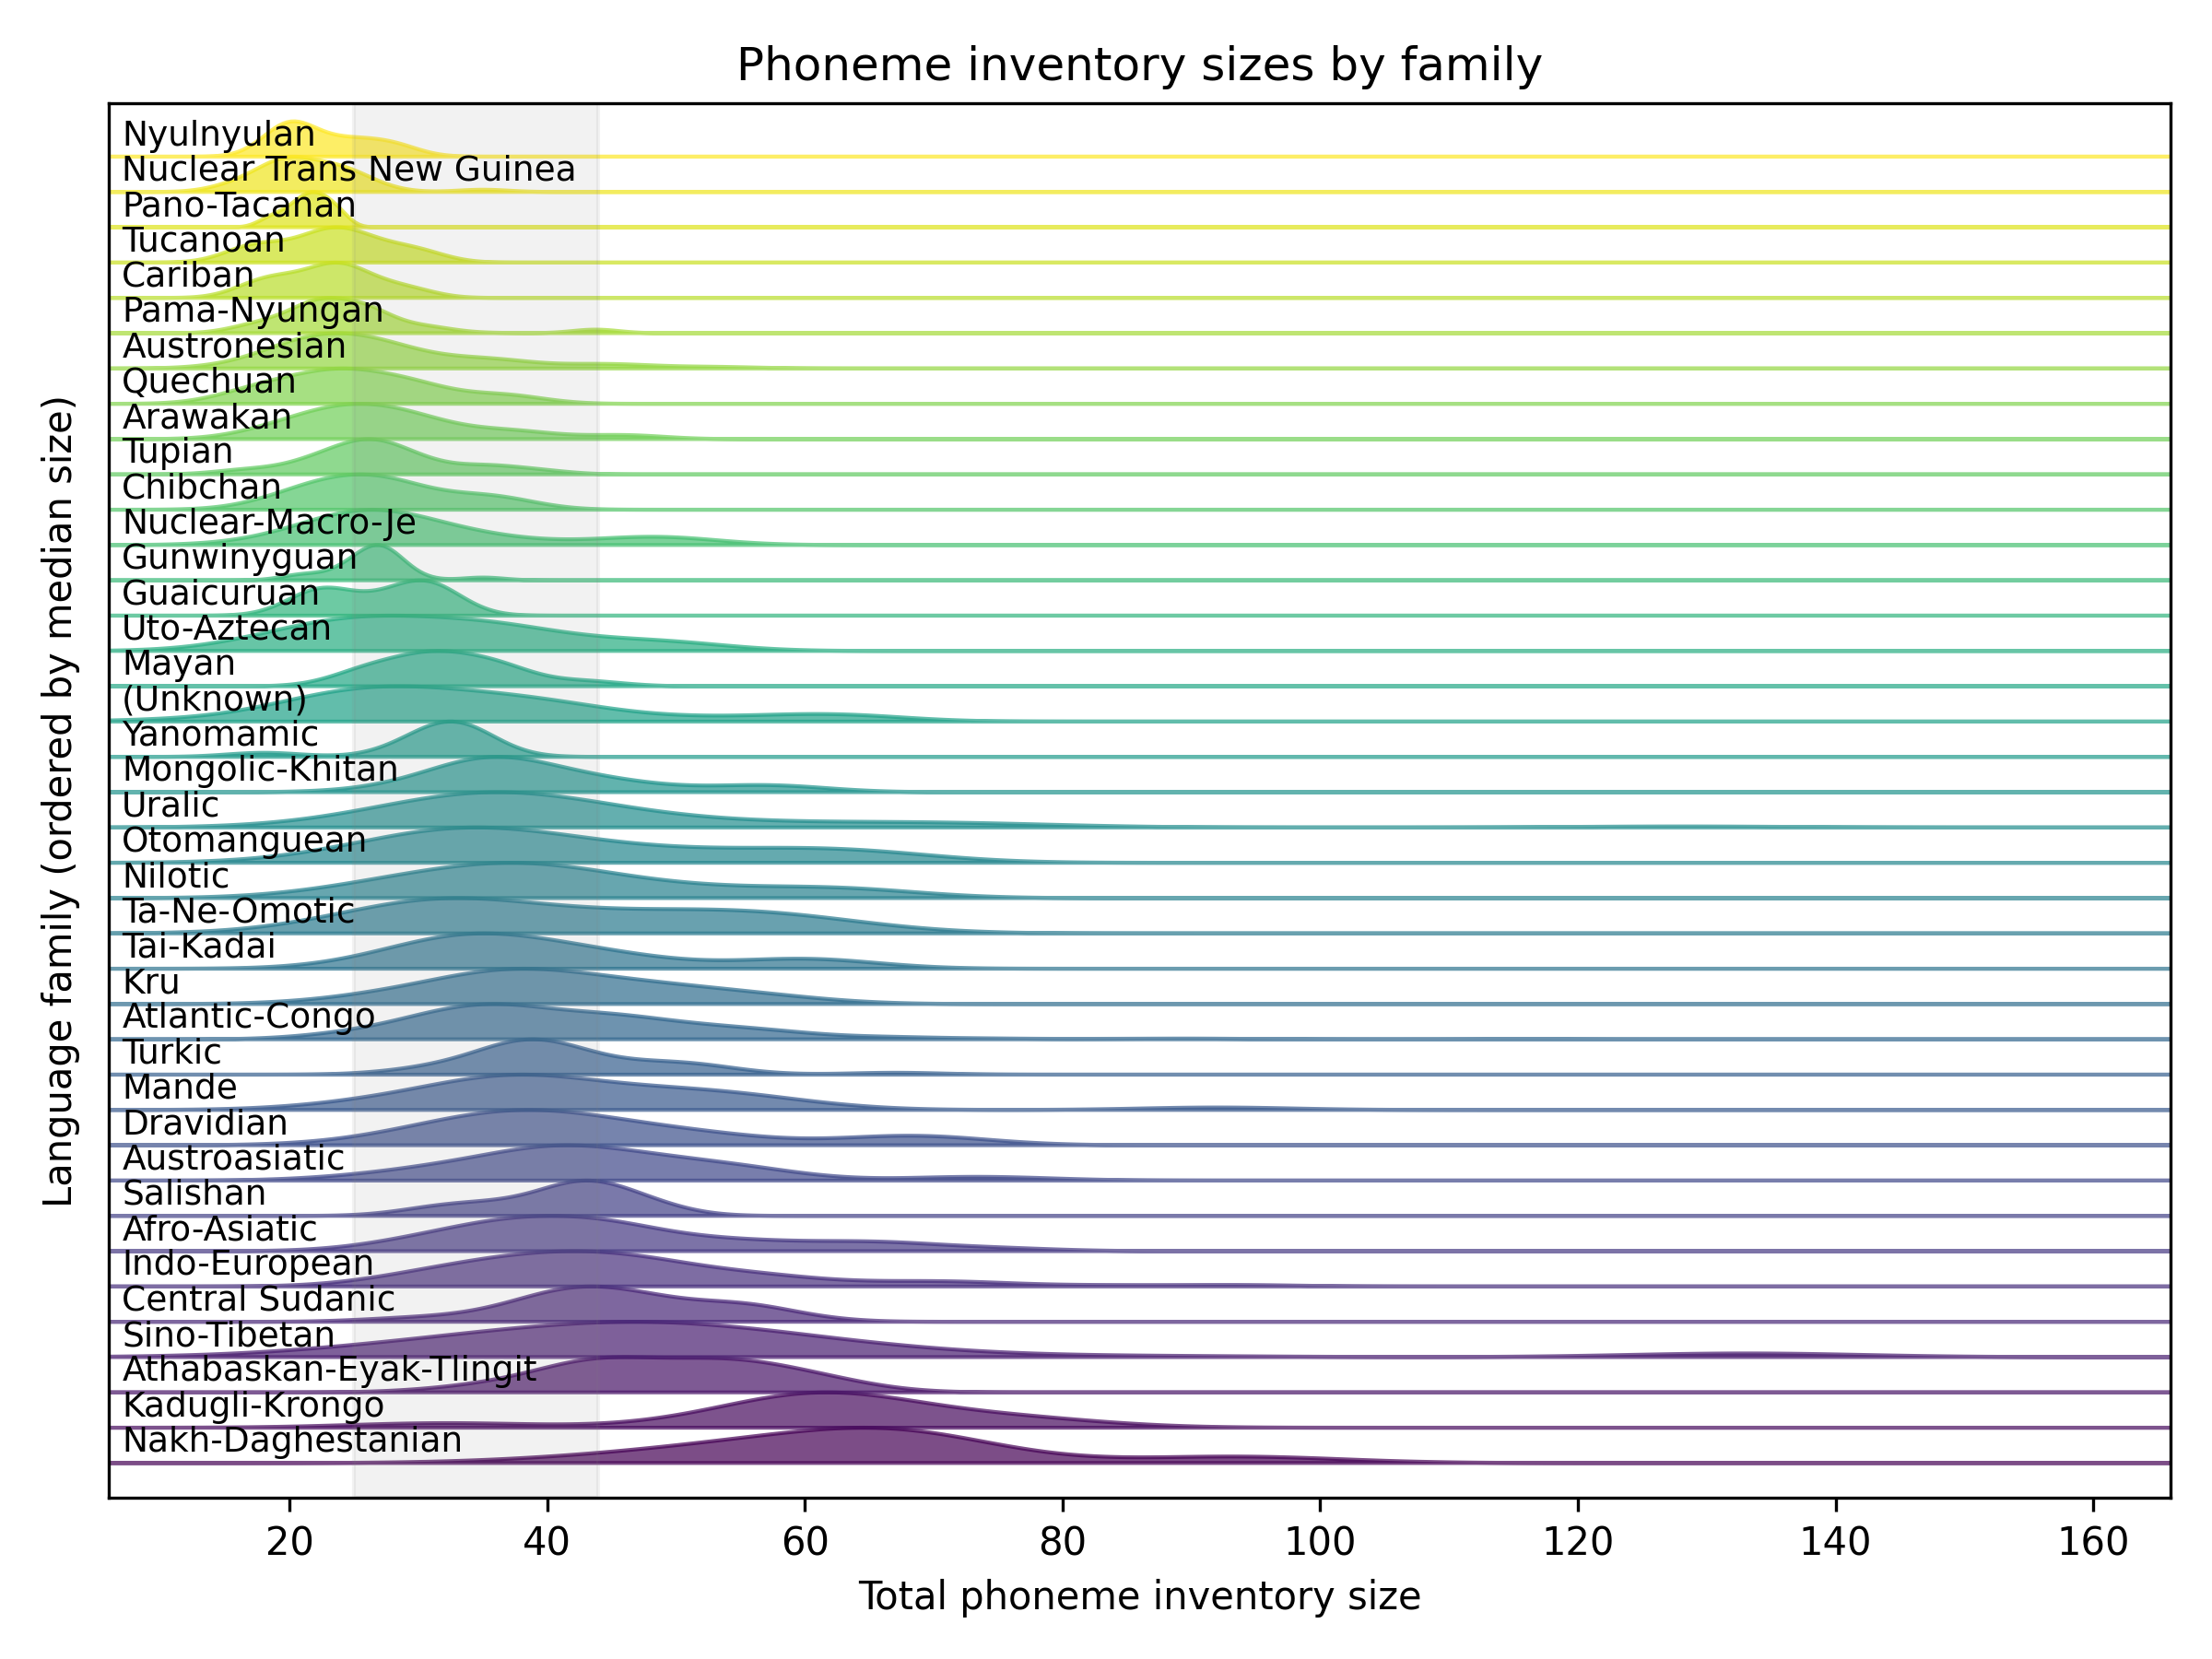
\includegraphics[width=\linewidth]{images/inventory_ridgelines.png}
  \caption{Phoneme inventory sizes by language family (PHOIBLE~2.0).
  Densities are shown for families with $n \ge 10$ languages, ordered by family median.
  Most families cluster in the 20–50 range (shaded), consistent with a homeostatic regime under articulatory–perceptual and dispersion constraints.
  Data: PHOIBLE~2.0; analysis code and exact processing steps are provided in the companion repository.}
  \label{fig:ridgelines}
\end{figure}

% --- Figure: P(/y/) vs vowel-inventory size (with /i/ comparison) ---
\begin{figure}[t]
  \centering
  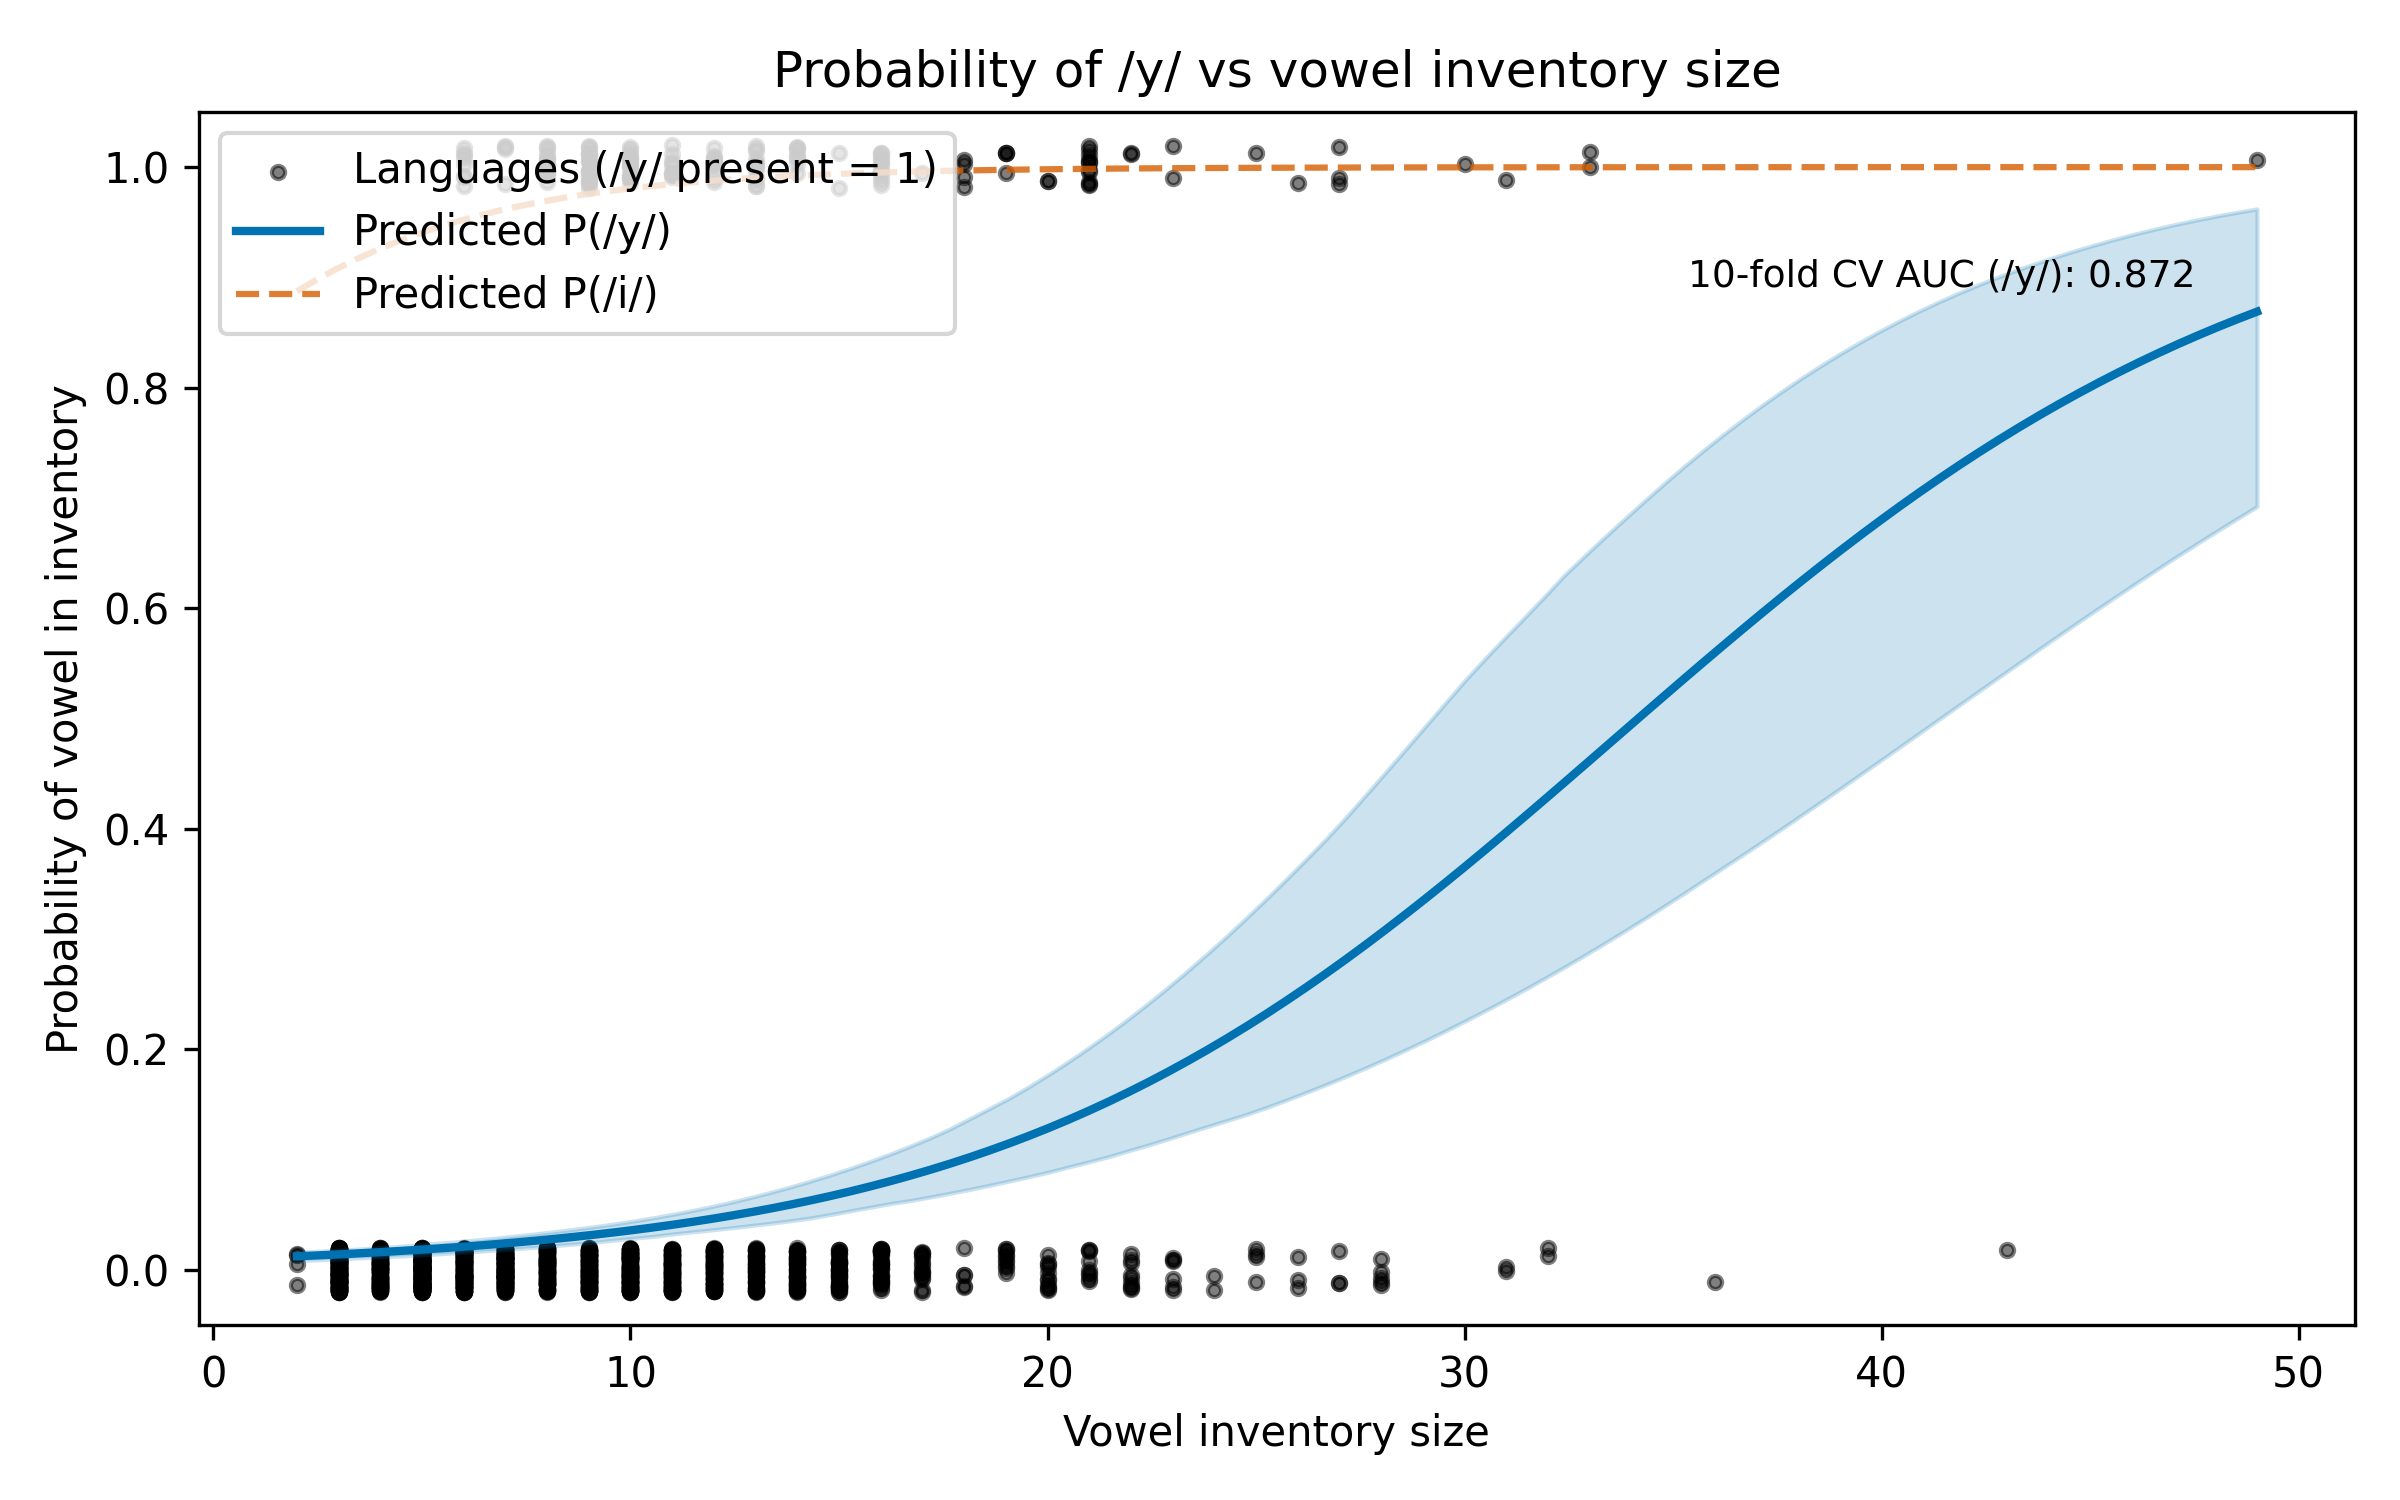
\includegraphics[width=\linewidth]{images/y_vs_vowel_inventory.png}
  \caption{Presence of /\textipa{y}/ as a function of vowel-inventory size.
  Solid line: logistic fit with 95\% CI ribbons; dashed line: comparison curve for /\textipa{i}/.
  Points are languages jittered vertically at 0/1 for presence/absence.
  Model includes a language-family effect; 10-fold cross-validation AUC is shown in-plot.
  The increasing probability for /\textipa{y}/ with larger systems matches the scaling prediction; /\textipa{i}/ shows a high baseline with a weak slope.}
  \label{fig:y-scaling}
\end{figure}


This article proposes a general, testable program: many linguistic categories---phonemes, lexemes, and language-internal constructions---are HPC kinds. The claim is operational, not merely analogical. I introduce two diagnostics and apply them across levels with compact, reproducible case studies, alongside a principled failure taxonomy that blocks over-generalization.

\emph{Diagnostic 1: Projectibility.} A proposed category is projectible if tokens support reliable out-of-sample inference about form, meaning, or distribution. This can be quantified with cross-corpus replication, held-out prediction, or cluster-cohesion under temporal or register shifts.

\emph{Diagnostic 2: Homeostasis.} A proposed category is homeostatic if its property cluster can be tied to specific stabilizers---biophysical attractors (e.g., quantal stability, dispersion), acquisition dynamics (e.g., perceptual magnets; sensorimotor adaptation), and sociocultural norms (local performance standards; entrenchment)---and if the expected covariance among properties can be demonstrated.

The first case study revisits the phoneme level using PHOIBLE-derived summaries but focuses on signatures rather than re-deriving physiology: inventory ridgelines by family and a logistic model for $P(\text{/y/})$ given inventory size, with family-wise subsampling as a sensitivity check. The HPC reading is straightforward: projectibility follows from the tight family distributions; homeostasis is underwritten by quantal stability and dispersion, with developmental tuning and community norms supplying the cultural scaffolding \citep{Ekstrom2025PhonemeTool}.

The second case study turns to words. Building on \citet{Miller2021WordsSpeciesKinds}, I track distributional drift for a single lexeme undergoing semantic change and show that a distributional neighborhood remains cohesive enough for decade-held-out prediction. Projectibility is demonstrated empirically; homeostasis is attributed to entrenchment and norm-guided usage that keep orthography/phonology/meaning covarying at usable levels, even as meanings shift.

The third case study treats an English construction, \emph{let alone}, as a language-internal HPC kind. Its cue bundle (string anchor, syntactic environment, conventionalized pragmatic contrast) yields robust extraction and cross-corpus replication; stabilizers include frequency, redundancy of cues, and normative enforcement (including editorial practices). Projectibility is tested by training on one corpus and predicting on another.

Equally important are the failure cases. Some proposals are too thin: one-off items (nonce coinages), performance blends, and child-only overregularizations within the adult standard lack the stabilizers that make inference sensible. Others are too fat: analyst-level macro-categories such as cross-linguistic ``resultative'' or ``ditransitive'' pool distinct local equilibria; the relevant mechanisms are local, so the global umbrella is not a single HPC kind. Finally, negative or complement classes (e.g., ``ungrammatical strings'') are defined by failure rather than by a causally sustained cluster. The discipline here is mechanism-first, in line with the word-kinds program \citep{Miller2021WordsSpeciesKinds}.

The framework yields predictions and disconfirmers. A perturbation prediction: weakening a stabilizer (e.g., lowering frequency or impoverishing input) will reduce cluster covariance before norms re-stabilize---a pattern testable under register shifts or in learner corpora. A scaling prediction: rarer but quantally robust members (e.g., /y/ in the vowel space) become more probable as system size grows; analogously, low-frequency constructional variants should be more prevalent in larger constructicons. Both predictions borrow directly from the phoneme results \citep[Fig.\,2 p.\,7]{Ekstrom2025PhonemeTool} and extend them to higher levels.

In sum, properly operationalized HPC naturalizes linguistic ontology for cognitive science. It tells us when a category is the right sort of thing to underwrite inference, what keeps it stable enough, and how it can change. At the phoneme level, the ridgeline and scaling patterns already instantiate homeostasis under constraint; at the word and construction levels, analogous signatures can be demonstrated with standard corpus methods. The result is not that everything is an HPC, but that many linguistic categories pass a disciplined test---and some do not \citep{Miller2021WordsSpeciesKinds,Ekstrom2025PhonemeTool}.

\section{Framework and diagnostics}\label{sec:framework}

The claim is ontological but operational. Following the homeostatic property–cluster (HPC) account of kinds \citep{Boyd1991Enthusiasm,Boyd1999Homeostasis}, with priority in \citet[§3.8]{Boyd1988MoralRealist} and explicit room for socially scaffolded kinds in \citet{Boyd2000Workmanship}, I take a linguistic kind to be a probabilistic cluster of properties whose stability over time and across a population is maintained by identifiable mechanisms. For words, this mechanism‐first stance has already been argued in detail: kindhood is earned a posteriori when internal and external stabilizers sustain covariation among pronunciation, orthography, meaning, and distribution so that speakers can project reliably from observed tokens to new ones \citep{Miller2021WordsSpeciesKinds}. I generalize that template across levels (phonemes, lexemes, and language‐internal constructions) and provide diagnostics that make the thesis adjudicable.

\subsection{Kinds in language as HPCs}

Let $K$ be a proposed linguistic category (e.g., \textit{/y/}, \textit{egregious}, the \textit{let alone} construction) over a population $P$ and time slice $T$. $K$ is an HPC kind for $\langle P,T\rangle$ iff:

\begin{enumerate}
\item tokens of $K$ instantiate a family of properties $C$ (articulatory/acoustic, semantic, distributional, prosodic, orthographic) that covary to a degree sufficient for inductive use; and
\item there exist mechanisms $M$ that, in fact, maintain that covariance in $\langle P,T\rangle$.
\end{enumerate}

The first condition is epistemic—do tokens support reliable out‐of‐sample inference? The second is metaphysical—what makes such inferences non‐accidental. Both are population‐ and time‐relative: kinds are discovered a posteriori, not fixed by essences \citep{Boyd1991Enthusiasm,Miller2021WordsSpeciesKinds}.

\subsection{Diagnostic 1: Projectibility}\label{sec:projectibility}

A category is projectible if it licenses reliable predictions about unseen tokens. We operationalize this with standard out‐of‐sample tests appropriate to each level:

\begin{itemize}
\item \textit{Phoneme tier.} Predict properties of inventories for held‐out languages or families (e.g., the probability that a system contains \textit{/y/} given vowel‐inventory size). Figures~\ref{fig:ridgelines}–\ref{fig:y-scaling} instantiate this with family‐wise ridgelines and a logistic curve for \textit{/y/}.
\item \textit{Word tier.} Track a lexeme’s distributional neighborhood across time and predict decade‐held‐out usage or sense‐proxies. Stable predictive performance under drift indicates projectibility \citep[mechanism‐first reading in][]{Miller2021WordsSpeciesKinds}.
\item \textit{Construction tier.} Train a cue‐bundle recognizer (string anchor, syntactic environment, typical collocates) on one corpus and test on another; cross‐corpus replication is the key signature.
\end{itemize}

Evidence is quantitative (AUC/accuracy for held‐out prediction; silhouette or cluster‐cohesion indices; replication across corpora/registers) and comparative (performance above baselines that ignore the putative stabilizers).

\subsection{Diagnostic 2: Homeostasis}\label{sec:homeostasis}

A category is homeostatic if we can name mechanisms that would sustain the observed covariance and then show the expected signatures of those mechanisms in the data. For language, the relevant stabilizers fall into three broad classes:

\begin{enumerate}
\item \textit{Biophysical constraints} (articulatory and auditory): quantal stability regions and dispersion pressures make certain segmental contrasts robust; these deliver the well‐known concentration of inventories and scaling of rarer vowels with system size \citep[their Fig.~1 and Fig.~2; Table~1]{Ekstrom2025PhonemeTool}.
\item \textit{Learning and control dynamics}: perceptual magnet effects, audio–motor adaptation, feedback control, and frequency‐based entrenchment bind cues within a category and damp variance.
\item \textit{Sociocultural norms}: locally taught performance standards, editorial practices, and interactional expectations shape distributions and prune unstable variants. Boyd’s extension to socially sustained kinds legitimizes these as part of the homeostatic base \citep{Boyd2000Workmanship}.
\end{enumerate}

Typical signatures include: (i) \emph{scaling laws} (e.g., increasing $P(\textit{/y/})$ with vowel‐inventory size), (ii) \emph{stability bands} (inventory sizes clustering in a narrow range by family), (iii) \emph{cue bundling and redundancy} (multiple partially overlapping cues for the same construction), and (iv) \emph{time‐series inertia} (slow drift with preserved covariance).

\subsection{Operational protocol}

To decide kindhood for $K$ in $\langle P,T\rangle$:

\begin{enumerate}
\item Specify the property set $C$ and the hypothesised stabilizers $M$ (drawn from the three classes above).
\item Run a projectibility assay suited to $K$ (held‐out prediction or cross‐corpus replication with baselines).
\item Test homeostasis by linking $M$ to data signatures: e.g., demonstrate a scaling relation; show lower within‐category variance for the cues $M$ predicts should covary; show covariance persists under drift or register shift.
\item Report failures. If projectibility is absent or no plausible $M$ can be named (or if predicted signatures are missing), withhold kindhood. This blocks “everything is an HPC.”
\end{enumerate}

\subsection{Delimiting scope}

Two guardrails follow from the diagnostics. First, kinds are \emph{local equilibria}. Cross‐linguistic umbrellas such as \textit{resultative} or \textit{ditransitive} usually pool distinct mechanisms; treat them as interest‐relative taxonomies, not single kinds. Second, negative/complement classes and one‐off items (nonce coinages, performance blends) lack stabilizers; they are not kinds.\footnote{For words, see \citet{Miller2021WordsSpeciesKinds}; for phonemes as culturally maintained cognitive tools with biophysical and social stabilizers, see \citet{Ekstrom2025PhonemeTool}.}

This framework aligns linguistic ontology with HPC realism: projectible clusters underwritten by concrete mechanisms rather than essences, historically and socially situated rather than timelessly fixed \citep{Boyd1991Enthusiasm,Boyd1999Homeostasis,Boyd2000Workmanship}.


\clearpage
\bibliographystyle{apalike}
\bibliography{refs}

\end{document}
